
\section{可点击图}

\begingroup
\def\pgfplotsmanualcurlibrary{clickable}
    \expandafter\ifx\csname pgfplotsclickabledisabled\endcsname\relax
    \else
        \pgfkeysdef{/pgfplots/clickable coords}{}%
        \pgfkeysdef{/pgfplots/clickable coords code}{}%
    \fi

\begin{pgfplotslibrary}{clickable}
    本库在点击图时生成小弹窗。弹窗显示鼠标指针所在位置的坐标，并支持可选的
    “吸附到最近点” |clickable coords| 特性，显示信息可自定义。此外，若按住鼠标
    并拖动到图中另一点，本库还可以显示斜率。

    本库有两个用途：以简单方式计算斜率\footnote{作者是应用数学家……}，以及为
    单个数据点提供相关的可选信息——这些信息重要性不足以列入正文（例如原型参数
    或其他技术细节）。
\end{pgfplotslibrary}


\subsection{概览}

在文档导言区写入如下语句即可：
%
\begin{codeexample}[code only]
\usepgfplotslibrary{clickable}
\end{codeexample}
%
\noindent 这会自动为每个图做好准备。

本库依赖 Acrobat JavaScript 与 \pdf{} 表单：每个图都会变成一个按钮。

    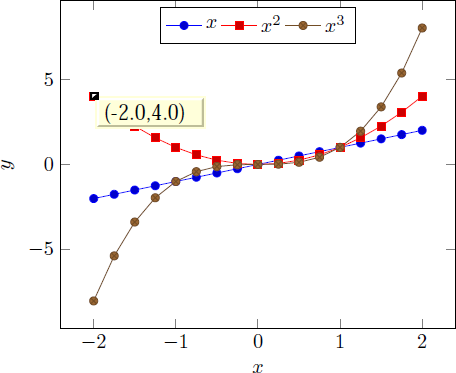
\includegraphics[height=6cm]{figures/pgfplotsclickable-fig1.png}
    \rlap{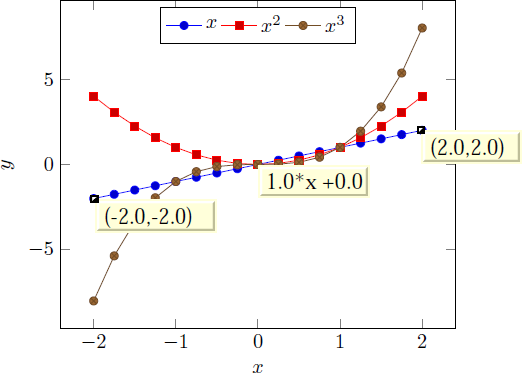
\includegraphics[height=6cm]{figures/pgfplotsclickable-fig2.png}}\hfill

\nobreak 这些截图展示了点击坐标轴范围（左列）以及从一点拖动到另一点（右列）的
结果。第二种情况展示了拖放的结果：它显示起点与终点，以及从拖动第一点到释放鼠标
第二点之间线段的方程。该线段为
%
    \[ l(x; x_0,y_0,x_1,y_1) = m \cdot x + n \]
%
其中 $m = (y_1-y_0) / (x_1-x_0)$ 为斜率，$n$ 为偏移量，其选取使得
$l(x_0;\dotsc) = y_0$。对于对数坐标图，会在计算斜率之前先取对数。

    \noindent
    \hbox to \linewidth{%
    \hspace{-0.5cm}%
    \begin{tikzpicture}
        \node at (8cm,0cm)    {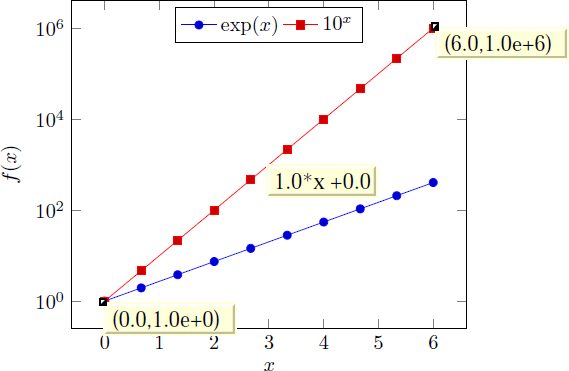
\includegraphics[height=6cm]{figures/pgfplotsclickable-fig4.png}};
        \node at (0cm,0cm)    {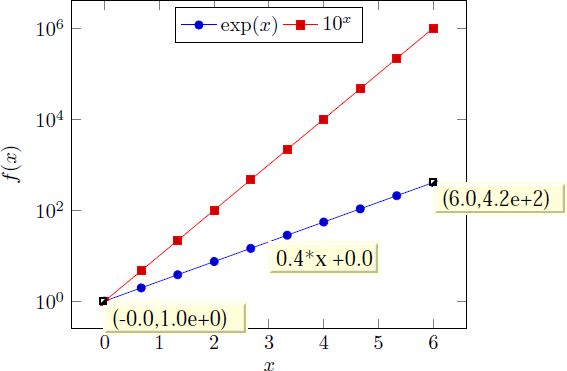
\includegraphics[height=6cm]{figures/pgfplotsclickable-fig3.png}};
    \end{tikzpicture}\hss}%

\nobreak 这些截图展示了\emph{对数}坐标轴下拖放的结果：端点再次显示坐标（不取对数），
中间的表单字段显示对数坐标下线性方程的斜率与偏移。

任何对数坐标轴的对数底通常为~$10$，但它会遵循 |log basis x| 与 |log basis y| 的
当前设置。所使用的对数与坐标轴描述所用的对数一致（这\emph{不一定}与
\PGFPlotstable{} 所用的相同！）。

本文档使用 |clickable| 库生成，因此可以在 Acrobat Reader 中打开它，直接点击图。

    \expandafter\ifx\csname pgfplotsclickabledisabled\endcsname\relax
    \else
    \paragraph{注意：}
    对于本文档，|clickable| 库已被禁用。你可以在
    \url{https://github.com/pgf-tikz/pgfplots} 上找到不同的版本。
    \fi

\begin{pgfplotskey}{clickable coords=\marg{displayed text}}
    点击绘图坐标时启用“吸附到最近点”特性。\meta{displayed text} 默认显示坐标的
    $x$ 与 $y$ 值（即你只需写 |clickable coords|，不带等号）。
    %
\begin{codeexample}[]
\begin{tikzpicture}
\begin{loglogaxis}[
    clickable coords={
        Level \thisrow{level} (q=\thisrow{q})
    },
]
    \addplot table [x=dof,y=error] {
        level  dof      error           q
        1      4        2.50000000e-01  48
        2      16       6.25000000e-02  25
        3      64       1.56250000e-02  41
        4      256      3.90625000e-03  8
        5      1024     9.76562500e-04  22
        6      4096     2.44140625e-04  46
        7      16384    6.10351562e-05  40
        8      65536    1.52587891e-05  3
        9      262144   3.81469727e-06  1
        10     1048576  9.53674316e-07  9
    };
\end{loglogaxis}
\end{tikzpicture}
\end{codeexample}
    %
    \noindent 现在，点击数据点会显示 `Level 7 (q=40)'，而点击数据点之外的地方
    则与之前一样显示点击坐标：

        \noindent\hbox to \linewidth{\hfill
        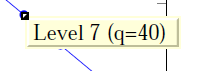
\includegraphics[scale=0.4]{figures/pgfplotsclickable-log-snap0}\hfill
        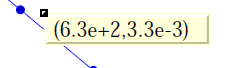
\includegraphics[scale=0.4]{figures/pgfplotsclickable-log-snap2}\hfill
        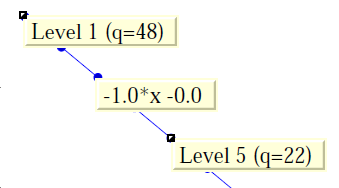
\includegraphics[scale=0.4]{figures/pgfplotsclickable-log-snap1}.\hfill
        }%

    注意，对数斜率的工作方式与之前相同。

    若希望显示 $(x,y)$ 值，请在 \meta{displayed text} 中使用特殊占位符
    `|(xy)|'。作为示例，再次考虑第~\pageref{pgfplots:scatterclasses} 页上的
    |scatter/classes| 例子：
    %
\begin{codeexample}[]
\begin{tikzpicture}
\begin{axis}[
    clickable coords={(xy): \thisrow{label}},
    scatter/classes={
        a={mark=square*,blue},
        b={mark=triangle*,red},
        c={mark=o,draw=black}   % <-- don't add comma
    }
]
    \addplot [
        only marks,
        scatter,
        scatter src=explicit symbolic
    ] table [meta=label] {
        x     y      label
        0.1   0.15   a
        0.45  0.27   c
        0.02  0.17   a
        0.06  0.1    a
        0.9   0.5    b
        0.5   0.3    c
        0.85  0.52   b
        0.12  0.05   a
        0.73  0.45   b
        0.53  0.25   c
        0.76  0.5    b
        0.55  0.32   c
    };
\end{axis}
\end{tikzpicture}
\end{codeexample}
    %
    \noindent 这里会看到类似如下的弹窗：

        \noindent\hbox to \linewidth{\hfill
        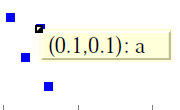
\includegraphics[scale=0.4]{figures/pgfplotsclickable-scatter1.png}\hfill
        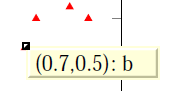
\includegraphics[scale=0.4]{figures/pgfplotsclickable-scatter2.png}\hfill
        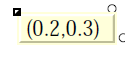
\includegraphics[scale=0.4]{figures/pgfplotsclickable-scatter0.png}.\hfill
        }%

    \meta{displayed text} 是一段富文本字符串，通过\emph{JavaScript}显示。
    对于大多数用途，它像未格式化的 C 字符串一样使用：包含字符，可能用 `|\n|'
    表示换行，或用 `|\t|' 表示制表符，但不应包含 \TeX{} 排版指令，尤其是数学模式
    （`|(xy)|' 替换文本由 |sprintf| 格式化，见下文）。若希望在显示前预处理数据，
    请考虑 |clickable coords code|。若遇到特殊字符问题，请尝试在其前面加反斜杠。
    若仍不行，尝试在单词前加 `|\\|' 和/或 `|\string|'。若要处理多行字段且需要
    调整大小分配，请考虑 |clickable coords size|。

    实际上，\meta{displayed text} 甚至可以包含富文本（即 XHTML）排版指令，如
    `|<br/>|'（注意末尾斜杠）或
    `|<span style="color:\#7E0000;">text</span>|'（注意 `|#|' 前的反斜杠），
    后者会改变 |text| 的颜色。|<span style="">| 的参数是 CSS 字段，CSS 属性列表
    请参考 HTML 文档。

    可以将 |clickable coords| 与三维坐标轴一起使用。注意，若三维坐标轴未设置
    |clickable coords|，其动态（可点击）特性将被禁用（因为它们似乎没用）。
    此外，三维坐标轴不支持斜率计算；只有“吸附到最近点”特性可用。

    可考虑使用 |annot/snap dist=6| 来增大“吸附到最近点”的距离。

    |clickable coords| 可以像上面的例子那样为坐标轴中的所有图指定，也可以为每个
    |\addplot| 命令分别指定（当希望对该命令使用“吸附到最近点”特性，并使用不同的
    \meta{displayed text} 时）。

    若多个 |clickable coords| 位于同一位置，每次点击会按出现顺序选择下一个。
\end{pgfplotskey}

\begin{pgfplotskey}{clickable coords code=\marg{%
    \TeX{} code which defines {\normalfont\ttfamily\textbackslash pgfplotsretval}}%
}
    这是 |clickable coords| 的一个变体，允许在将显示信息交给 JavaScript 之前
    对其进行预处理。

    该值应为 \TeX{} 代码，以某种方式定义 |\pgfplotsretval|。结果用作与坐标关联的
    简单未格式化字符串。

    可考虑使用

    \hspace{2em}|\pgfmathprintnumberto[verbatim]|\marg{number}|\macroname|

    \hspace{2em}|\edef\pgfplotsretval{Number=\macroname}|

    来提供数字打印。|\pgfmathprintnumberto[verbatim]| 不使用数学模式格式化
    数字，\footnote{数字打印的细节见 \PGFPlotstable{} 手册。}
    并将结果写入 |\macroname|。名称 `|\macroname|' 是任意的，可使用
    `|\eps|' 或 `|\info|' 之类。|\edef| 表示“展开定义”，其效果是展开所有宏以
    确定值，在本例中即“Number = \meta{the value}”。下面的例子使用它两次来美观地
    打印数据：
    %
\begin{codeexample}[]
\begin{tikzpicture}
\begin{loglogaxis}[clickable coords code={
    \pgfmathprintnumberto[verbatim,precision=1]
        {\thisrow{error}}
        \error
    \pgfmathprintnumberto[verbatim,frac]
        {\thisrow{frac}}
        \fraccomp
    \edef\pgfplotsretval{error \error, R=\fraccomp}
}]
    \addplot table [x=dof,y=error] {
        level  dof     error           frac
        1      4       2.50000000e-01  0.5
        2      16      6.25000000e-02  0.75
        3      64      1.56250000e-02  0.1
        4      256     3.90625000e-03  0.2
        5      1024    9.76562500e-04  0.5
        6      4096    2.44140625e-04  0.8
        7      16384   6.10351562e-05  0.125
        8      65536   1.52587891e-05  0.725
        9      262144  3.81469727e-06  0.625
        10     1048576 9.53674316e-07  1
    };
\end{loglogaxis}
\end{tikzpicture}
\end{codeexample}
    %
    \noindent 结果为

        \noindent\hbox to \linewidth{\hfill
        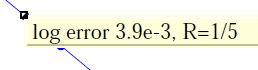
\includegraphics[scale=0.4]{figures/pgfplotsclickable-logcode-snap0.png}\hfill
        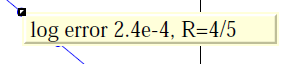
\includegraphics[scale=0.4]{figures/pgfplotsclickable-logcode-snap1.png}.\hfill
        }%

    \meta{\TeX{} code} 在局部作用域内求值，之后所有局部声明的变量都会被释放
    （因此可以使用任意名称）。
\end{pgfplotskey}

\begin{pgfplotskey}{%
    clickable coords size=\texttt{auto} or \marg{max chars} or
    \marg{max chars x,max chars y} (initially auto)%
}
    这实际上就是 |annot/popup size snap| 的另一个名称，见下文其文档。
\end{pgfplotskey}


\subsection{库的要求}

\begin{itemize}
    \item 本库依赖 \LaTeX{} 宏包 |insdljs|（“Insert document level JavaScript”）
        与 |eforms|，二者均属于免费的 |AcroTeX| 教育套件~\cite{acrotex}。
        \footnote{这些宏包依赖 \LaTeX{}，因此本库仅适用于 \LaTeX{}，
        不适用于 plain \TeX{} 或 Con\TeX{}t。}
        |insdljs| 宏包会创建一个扩展名为 |.djs| 的临时文件。
    \item 在撰写本文时，只有 Adobe Acrobat Reader 能正确解释 JavaScript 与表单。
        据我所知，若生成的文档在其他阅读器中使用，本库不会产生任何效果。
\end{itemize}
%
注意，虽然本库是为 \PGFPlots{} 编写的，但它可以独立于 \PGFPlots{} 环境使用。


\paragraph{兼容性问题：}

使用本库时有若干限制。其中大部分将在未来版本中消失——但到目前为止，我无法
施展魔法。
%
\begin{itemize}
    \item 本库尚不支持旋转坐标轴。对这些坐标轴请使用 |clickable=false|。
    \item 本库仅适用于 |pdflatex|；不支持 |dvips| 或 |dvipdfm|。
        \footnote{实际上它们应该可以支持。我并不确知为何不行。欢迎提供线索。}
    \item 到目前为止，\emph{无法}将本库与 |external| 库及第~\ref{cha:pgfplots:importexport}
        章中的其他图像外部化方法一起使用。

        更准确地说，你可以（通过两行额外导言代码，见下）得到正确标注、导出的
        \pdf{} 文档，但 |\includegraphics| 命令不会导入动态特性。

        若决定使用此变通方法，需要在加载 \pgfname{}、\Tikz{} 或 \PGFPlots{}
        \emph{之前}插入
        %
\begin{codeexample}[code only]
% \maxdeadcycles=10000 % in case you get the error `Output loop---<N> consecutive dead cycles.'
\usepackage[pdftex]{eforms}
\end{codeexample}
        %
        \noindent。|\maxdeadcycles| 对于大型文档似乎是必要的，请尝试一下。

        在编写文档草稿期间，你可能希望在导言区使用
        %
\begin{codeexample}[code only]
\pgfkeys{/pgf/images/include external/.code={\href{file:#1}{\pgfimage{#1}}}}
\end{codeexample}
        %
        这会在图形文件周围生成超链接，链接到导出的图片。点击超链接会打开导出的
        图片，而该图片本身是用 |clickable| 库生成的，因而支持动态特性。
        \footnote{这种特殊处理要求外部文件与主文档位于同一基目录，因此这种方法
        \emph{肯定}不适用于最终文档。}
    \item 本库会在 |\begin{document}| 处自动调用 |\begin{Form}|，并在文档末尾调用
        |\end{Form}|。hyperref 的该环境对于动态用户交互是必要的，若文档包含其他
        表单元素，请记住这一点。
\end{itemize}

\paragraph{致谢：}

\begin{itemize}
    \item 我使用了 Kevin van Zonneveld 的 JavaScript |sprintf| 实现~\cite{phptojs}
        （JavaScript API 仅提供有限的转换集合）。
\end{itemize}


\subsection{自定义}

可以通过若干选项自定义本库。

\begin{pgfplotskey}{clickable=\mchoice{true,false} (initially true)}
    允许对单个图禁用本库。
\end{pgfplotskey}

\begin{pgfplotskey}{annot/js fillColor=\marg{JavaScript color} (initially ["RGB",1,1,.855])}
    设置短弹窗注释的背景（填充）颜色。

    可选值为 |transparent|、灰色、RGB 或 CMYK 颜色，以四元素数组形式指定，形如
    |["RGB", |\meta{red}|,|\meta{green}|,|\meta{blue}|]|。每个颜色分量介于
    $0$ 与 $1$ 之间。

    再次强调：该选项用于 JavaScript。\emph{不能}像在 \pgfname{} 中那样使用颜色。
\end{pgfplotskey}

\begin{pgfplotskeylist}{%
    annot/point format=\marg{sprintf-format} (initially {(\%.1f,\%.1f)}),
    annot/point format 3d=\marg{sprintf-format} (initially {(\%.1f,\%.1f,\%.1f)})%
}
    允许提供 |sprintf| 格式字符串，用于填充注释文本。|sprintf| 的第一个参数为
    $x$ 坐标，第二个参数为 $y$ 坐标。

    |point format 3d| 变体用于任何三维坐标轴，而 |point format|（仅）用于二维坐标轴。

    |every semilogx axis|、|every semilogy axis| 与 |every loglog axis| 样式已更新为
    %
\begin{codeexample}[code only]
\pgfplotsset{
    every semilogy axis/.append style={/pgfplots/annot/point format={(\%.1f,\%.1e)}},
    every semilogx axis/.append style={/pgfplots/annot/point format={(\%.1e,\%.1f)}},
    every loglog axis/.append style={/pgfplots/annot/point format={(\%.1e,\%.1e)}},
}
\end{codeexample}
    %
    \noindent 从而每个对数坐标都以科学计数法显示。
\end{pgfplotskeylist}

\begin{pgfplotskey}{annot/slope format=\marg{sprintf-format} (initially \%.1f*x \%+.1f)}
    允许提供 |sprintf| 格式字符串，用于填充斜率注释文本。第一个参数为斜率，
    第二个为直线偏移。
\end{pgfplotskey}

\begin{pgfplotskey}{annot/printable=\mchoice{true,false} (initially false)}
    用于配置是否打印小注释。否则它们仅在屏幕上可见。
\end{pgfplotskey}

\begin{pgfplotskey}{annot/font=\marg{JavaScript font name} (initially font.Times)}
    用于为注释选择 JavaScript 字体。可选项限于 JavaScript 所接受的范围
    （\emph{不}与 \LaTeX{} 相同）。默认字体及其名称如下所示。

    \begin{center}
        \begin{tabular}{ll}
                \toprule
            字体名称             & JavaScript 中的名称 \\
                \midrule
            Times-Roman           & font.Times         \\
            Times-Bold            & font.TimesB        \\
            Times-Italic          & font.TimesI        \\
            Times-BoldItalic      & font.TimesBI       \\
            Helvetica             & font.Helv          \\
            Helvetica-Bold        & font.HelvB         \\
            Helvetica-Oblique     & font.HelvI         \\
            Helvetica-BoldOblique & font.HelvBI        \\
            Courier               & font.Cour          \\
            Courier-Bold          & font.CourB         \\
            Courier-Oblique       & font.CourI         \\
            Courier-BoldOblique   & font.CourBI        \\
            Symbol                & font.Symbol        \\
            ZapfDingbats          & font.ZapfD         \\
                \bottomrule
        \end{tabular}
    \end{center}
\end{pgfplotskey}

\begin{pgfplotskey}{annot/textSize=\marg{Size in Point} (initially 11)}
    设置注释的文字大小，单位为磅。
\end{pgfplotskey}

\begin{pgfplotskeylist}{%
    annot/popup size generic=\texttt{auto} or \marg{x} or \marg{x,y} (initially auto),
    annot/popup size snap=\texttt{auto} or \marg{x} or \marg{x,y} (initially auto),
    annot/popup size=\marg{value}%
}
    第一个键定义仅点击坐标轴时弹窗的大小。第二个键定义“吸附到最近点”特性
    （即由 |clickable coords| 准备的那些）的弹窗大小。第三个键将二者设为相同的
    \meta{value}。

    参数可以为 |auto|，此时 \PGFPlots{} 会尝试智能地统计字符数。这对多行文本
    可能失败。选项 \meta{x} 仅提供\emph{水平}大小，单位为 |annot/textSize|。
    因此，|annot/popup size generic=6| 使弹窗宽为 $6\cdot 11$ 磅。此时只分配一行。
    最后，\meta{x,y} 允许提供水平与竖直大小，均以 |annot/textSize| 为单位。

    另见 |clickable coords size|，它是 |annot/popup size snap| 的别名。
\end{pgfplotskeylist}

\begin{pgfplotskey}{annot/snap dist=\marg{Size in Point} (initially 4)}
    定义两次鼠标点击被视为等价的距离，以磅为单位（欧氏距离）。
\end{pgfplotskey}

\begin{pgfplotskey}{annot/richtext=\mchoice{true,false} (initially true)}
    启用或禁用 |clickable coords| 参数中的富文本排版。富文本类似于 XHTML，
    允许使用 CSS 样式，如颜色、字体变化及其他 CSS 属性，细节见 |clickable coords|
    文档。

    |annot/richtext=false| 的情况可能更稳健。
\end{pgfplotskey}


\subsection{在其他场合使用可点击库}

本库本质上提供一个命令 |\pgfplotsclickablecreate|，它创建一个预定义大小的可点击
区域，并结合 JavaScript 交互代码。它可以独立于 \PGFPlots{} 使用。

\begin{command}{\pgfplotsclickablecreate\oarg{required key-value-options}}
    创建一个可点击区域。点击会产生一个弹窗，其中包含光标所在点的信息。

    完整（！）的上下文需要通过键值对提供，既可以在调用本方法之前设置，也可以在
    \oarg{required key-value-options} 内设置。

    该命令实际上创建一个 AcroForm，点击时调用 JavaScript。它会创建一个表示上下文
    （坐标轴范围与选项）的 JavaScript 对象。该 JavaScript 对象在运行时可用。

    本方法是公开的，\emph{不}限于 \PGFPlots{} 使用。\PGFPlots{} 的钩子只是初始化
    所需的键值对。

    本方法不绘制任何内容。它仅初始化可点击区域与 JavaScript 代码。

    所需的键值对见下文文档。

    \paragraph{注意：}

    这里\emph{不会}执行完整的键值校验。可能出现无效选项在 Acrobat Reader 中打开时
    产生 JavaScript 错误。请使用 JavaScript 控制台查找它们。
\end{command}

\noindent 以下所有选项仅对希望在不使用 \PGFPlots{} 的情况下使用本库的用户有意义。

\begin{pgfplotskey}{annot/width=\marg{dimension} (initially -)}
    该必需键将区域宽度传达给 |\pgfplotsclickablecreate|。它必须是 \TeX{} 尺寸，
    如 |5cm|。
\end{pgfplotskey}

\begin{pgfplotskey}{annot/height=\marg{dimension} (initially -)}
    该必需键将区域高度传达给 |\pgfplotsclickablecreate|。它必须是 \TeX{} 尺寸，
    如 |5cm|。
\end{pgfplotskey}

\begin{pgfplotskey}{annot/jsname=\marg{string} (initially -)}
    该必需键将唯一标识符传达给 |\pgfplotsclickablecreate|。该标识符用于在
    JavaScript 中标识对象，因此不能有多个。若为空，将生成默认标识符。
\end{pgfplotskey}

\begin{pgfplotskeylist}{%
    annot/xmin=\marg{number},
    annot/xmax=\marg{number},
    annot/ymin=\marg{number},
    annot/ymax=\marg{number} (initially empty)%
}
    这些必需键将坐标轴范围传达给 |\pgfplotsclickablecreate|。它们应设置为
    可赋值给 JavaScript 浮点数（标准 IEEE 双精度）的数字。
\end{pgfplotskeylist}

\begin{pgfplotskey}{annot/collected plots=\marg{nested arrays} (initially empty)}
    实现“吸附到最近点”特性的底层接口。其值为图的数组，每个图又是坐标的数组，
    而每个坐标是 $x$、$y$ 与文本三个元素的数组。细节与示例请参考代码注释。
\end{pgfplotskey}
\endgroup
